\documentclass[12pt,a4paper]{article}

\usepackage{tikz,amsmath,amssymb,amsfonts,cancel}

\author{Yuri Santos Silva}
\date{12, Março de 2025}
\title{Lista de exercício I}

\begin{document}
\maketitle
\vspace*{.5cm}

1 - Apresente uma parametrização para as seguintes curvas:

a) \( \gamma = \{ (x,y) \in \mathbb{R}^2; x = y^2, 0 \leq x \leq 5 \} \)
\[
  \gamma = (x,\sqrt{x}) = x\ \hat{i} + \sqrt{x}\ \hat{j};\ x \in [0;\ 5]
\]

b) \( \gamma = \{ (x,y) \in \mathbb{R}^2; x^2 + y^2 = 16; y > 0 \} \)
\[
  \gamma(\theta) = r\cos \theta\ \hat{i} + r\sin \theta\ \hat{j} = 4 \cos \theta\ \hat{i} + 4 \sin \theta\ \hat{j}; \theta \in [0,\ \pi]
\]

c) \( \gamma = \{ (x,y) \in \mathbb{R}^2; 3x + 2y - 5 = 0 \} \)
\[
  \gamma = 3x + 2\left[ \frac{5-3x}{2} \right] - 5 = 0; x \in \mathbb{R} \land y = \frac{5-3x}{2}
\]

d) \( \gamma \) é o segmento de reta que liga os pontos \( A = (-1,2,0) \) e \( B = (1,3,4) \)
\[
  r = B - A = [1 - (-1), 3 - 2, 4 - 0] = (2, 1, 4)
\]
\[
  \gamma = A + rx \implies (-1,2,0) + (2,1,4)x;\ x \in \mathbb{R}
\]
  
2) Esboce a curva usando as equações paramétricas para marcar os pontos. Indique com uma seta a direção na qual a curva é traçada quando t aumenta.

a) \( x = 1 + \sqrt{t}; y = t^2 - 4t; 0 \leq t \leq 5 \)
\[
  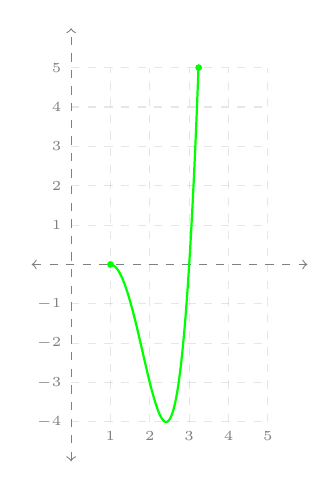
\begin{tikzpicture}[domain=0:5,smooth,samples=500,scale=.5]
    \draw[dashed,gray,<->] (0,-5) -- (0,6);
    \draw[dashed,gray,<->] (-1,0) -- (6,0);
    
    \foreach \x in {1,2,...,5}
    \draw[dashed,gray,opacity=.2] (\x,-4) -- (\x,5) node[anchor=north,pos=0,opacity=1]{\tiny$\x$};
    \foreach \x in {-4,...,-1,1,2,...,5}
    \draw[dashed,gray,opacity=.2] (0,\x) -- (5,\x) node[pos=0,anchor=east,opacity=1]{\tiny$\x$};

    \draw[green,thick] plot({1 + sqrt(\x)}, {\x * \x - 4 * \x});
    \draw[fill,green] (1,0) circle (2pt);
    \draw[fill,green] (3.24,5) circle (2pt);
  \end{tikzpicture}
\]

b) \( x = \cos^2 t; y =  1 - \sin t; 0\leq t \leq \frac{\pi}{2} \)
\[
  \begin{tikzpicture}[domain=0:3.14,samples=500,smooth]
    \draw plot ({(cos(\x r))^2},{1 - sin (\x) r});
  \end{tikzpicture}
\]


\end{document}